%%%%%%%%%%%%%%%%%%%%%%%%%%%%% Define Article %%%%%%%%%%%%%%%%%%%%%%%%%%%%%%%%%%
\documentclass[a4paper,11pt]{article}
%%%%%%%%%%%%%%%%%%%%%%%%%%%%%%%%%%%%%%%%%%%%%%%%%%%%%%%%%%%%%%%%%%%%%%%%%%%%%%%
\usepackage[utf8]{inputenc}
\usepackage[T1]{fontenc}
\usepackage{helvet}
\renewcommand{\familydefault}{\sfdefault}
%%%%%%%%%%%%%%%%%%%%%%%%%%%%% Using Packages %%%%%%%%%%%%%%%%%%%%%%%%%%%%%%%%%%
\usepackage{graphicx}
\usepackage{amssymb}
\usepackage{amsmath}
\usepackage{amsthm}
\usepackage{empheq}
\usepackage{mdframed}
\usepackage{booktabs}
\usepackage{lipsum}
\usepackage{graphicx}
\usepackage{color}
\usepackage{psfrag}
\usepackage{pgfplots}
\usepackage{bm}
%%%%%%%%%%%%%%%%%%%%%%%%%%%%%%%%%%%%%%%%%%%%%%%%%%%%%%%%%%%%%%%%%%%%%%%%%%%%%%%
\usepackage[colorlinks=true]{hyperref}
\hypersetup{
    colorlinks=true,
    linkcolor=blue!50!black,
    filecolor=blue!50!black,
    citecolor = green!50!black,      
    urlcolor=cyan,
}
\usepackage{fancyhdr}
\usepackage{amsmath}
\usepackage{amsthm}
\usepackage{empheq}
\usepackage{bm}
\usepackage{tikz}
\usepackage{subcaption}
\usepackage{multicol}
\usepackage{authblk}
\usepackage[left=3cm,right=3cm,top=2cm,bottom=2cm]{geometry}
\newcommand{\avg}[1]{\left<#1\right>}
\newcommand{\avgcond}[1]{\overline{#1}}
\newcommand{\oneavg}[1]{\avgcond{#1}^1}


% Other Settings
%%%%%%%%%%%%%%%%%%%%%%%%%% Page Setting %%%%%%%%%%%%%%%%%%%%%%%%%%%%%%%%%%%%%%%

\usepackage{natbib}
\bibliographystyle{plain}
\usepackage{enumitem}
\setlist{nolistsep}
%%%%%%%%%%%%%%%%%%%%%%%%%% Define some useful colors %%%%%%%%%%%%%%%%%%%%%%%%%%
\definecolor{ocre}{RGB}{243,102,25}
\definecolor{mygray}{RGB}{243,243,244}
\definecolor{deepGreen}{RGB}{26,111,0}
\definecolor{shallowGreen}{RGB}{235,255,255}
\definecolor{deepBlue}{RGB}{61,124,222}
\definecolor{shallowBlue}{RGB}{235,249,255}
%%%%%%%%%%%%%%%%%%%%%%%%%%%%%%%%%%%%%%%%%%%%%%%%%%%%%%%%%%%%%%%%%%%%%%%%%%%%%%%

%%%%%%%%%%%%%%%%%%%%%%%%%% Define an orangebox command %%%%%%%%%%%%%%%%%%%%%%%%
\newcommand\orangebox[1]{\fcolorbox{ocre}{mygray}{\hspace{1em}#1\hspace{1em}}}
%%%%%%%%%%%%%%%%%%%%%%%%%%%%%%%%%%%%%%%%%%%%%%%%%%%%%%%%%%%%%%%%%%%%%%%%%%%%%%%

%%%%%%%%%%%%%%%%%%%%%%%%%%%% English Environments %%%%%%%%%%%%%%%%%%%%%%%%%%%%%
\newtheoremstyle{mytheoremstyle}{3pt}{3pt}{\normalfont}{0cm}{\rmfamily\bfseries}{}{1em}{{\color{black}\thmname{#1}~\thmnumber{#2}}\thmnote{\,--\,#3}}
\newtheoremstyle{myproblemstyle}{3pt}{3pt}{\normalfont}{0cm}{\rmfamily\bfseries}{}{1em}{{\color{black}\thmname{#1}~\thmnumber{#2}}\thmnote{\,--\,#3}}
\theoremstyle{mytheoremstyle}
\newmdtheoremenv[linewidth=1pt,backgroundcolor=shallowGreen,linecolor=deepGreen,leftmargin=0pt,innerleftmargin=20pt,innerrightmargin=20pt,]{theorem}{Theorem}[section]
\theoremstyle{mytheoremstyle}
\newmdtheoremenv[linewidth=1pt,backgroundcolor=shallowBlue,linecolor=deepBlue,leftmargin=0pt,innerleftmargin=20pt,innerrightmargin=20pt,]{definition}{Definition}[section]
\theoremstyle{myproblemstyle}
\newmdtheoremenv[linecolor=black,leftmargin=0pt,innerleftmargin=10pt,innerrightmargin=10pt,]{problem}{Problem}[section]
%%%%%%%%%%%%%%%%%%%%%%%%%%%%%%%%%%%%%%%%%%%%%%%%%%%%%%%%%%%%%%%%%%%%%%%%%%%%%%%

%%%%%%%%%%%%%%%%%%%%%%%%%%%%%%%%%%%%%%%%%%%%%%%%%%%%%%%%%%%%%%%%%%%%%%%%%%%%%%%
\fancyhead[L]{
\includegraphics[scale=1]{image/logo.png}}

%%%%%%%%%%%%%%%%%%%%%%%%%%%%%%% Title & Author %%%%%%%%%%%%%%%%%%%%%%%%%%%%%%%%
% \title{{\Large  Toward a generalized hydrodynamic drag law for cylinder particles, Suspensions dynamics of cylindrical particles,} }
\author{\large GAMET Lionel}
\author{\large PIERSON Jean-Lou}
\author{\large GAMET Lionel$^1$, PIERSON Jean-Lou$^2$ and FINTZI Nicolas$^3$}
%%%%%%%%%%%%%%%%%%%%%%%%%%%%%%%%%%%%%%%%%%%%%%%%%%%%%%%%%%%%%%%%%%%%%%%%%%%%%%%
\newcommand{\size}{0.6}
\begin{document}
\begin{flushright}
    FINTZI Nicolas
    
    nicolas.fintzi@ifpen.fr
\end{flushright}
\begin{center}
    % \normalsize \hrule height 0.3ex \vspace{0.2ex} \hrule height 0.1ex
    \vspace{10pt}
    {\Large Theoretical calculation of the droplet induced agitation (or pseudoturbulence) in buoyant emulsions in the low inertia and dilute regimes.}\\
    \vspace{10pt}
    % \normalsize \hrule height 0.1ex \vspace{0.2ex} \hrule height 0.3ex

    \vspace{15pt}
    {\large FINTZI Nicolas$^{1,2}$, PIERSON Jean-Lou$^1$ and POPINET St\'ephane$^2$}
\end{center}
% \maketitle

\begin{flushleft}
$^{1}$\large IFP Energies Nouvelles, Rond-point de l’echangeur de Solaize, 69360 Solaize.

$^{2}$\large Sorbonne Universit\'e, Institut Jean le Rond d'Alembert, 4 place Jussieu, 75252 PARIS CEDEX 05, France.

fintzi.nicolas@ifpen.fr 

jean-lou.Pierson@ifpen.fr

stephane.popinet@upmc.fr

% Lionel.Gamet@ifpen.fr

\end{flushleft}
\begin{itemize}
\item Communication preference : Oral presentation;
\item Keywords : Hydrodynamics, Averaged equations, Pseudoturbulence, Stokes flows;
\item Speaker : FINTZI Nicolas / nicolas.fintzi@ifpen.fr
\end{itemize}


\vspace{15pt}

Buoyancy-driven droplet flows are encountered in many chemical engineering processes such as gravity separators and liquid-liquid extractors. 
The usual engineering practice to model such facilities is to use the averaged Navier-Stokes equations. 
The present work focuses on the velocity fluctuations tensor, also known as the \textit{Reynolds stress} tensor, or Pseudo-turbulent tensor, which is a crucial closure term in these equations.
Formally, this stress is defined as $\avg{ \textbf{u}' \textbf{u}'}_f$, where $\textbf{u}'$ is the fluid velocity fluctuation, and $\avg{\ldots}_f$ denotes an ensemble average procedure applied over the continuous phase. 
The \textit{Reynolds stress} can be separated into two contributions : (1) The agitation generated due to the averaged wakes around the particles; (2) All other sources of fluctuations, such as those generated through particle interactions, and single-phase turbulence \cite{du2022analysis}.
This study only considers the first contribution. 
Specifically we compute $\avg{ \textbf{u}' \textbf{u}'}_f$, for buoyant rising droplets in an otherwise quiescent fluid. 
The derivation is restricted to spherical droplets (of radius $a$), at small particle Reynolds number, and low particle volume fraction ($\phi$). 


For buoyant inviscid bubbly flows under the dilute assumption, it is known since the study of \cite{van1982bubble} that the \textit{Reynolds stress} can be written as
\begin{equation}
    \avg{\textbf{u}'\textbf{u}'}_f (\textbf{x})
    \approx
    n_p \int_{|\textbf{r}| > a}\textbf{v}\textbf{v}  d\textbf{r}
    = \phi \left(\frac{3}{20} U^2\textbf{I} + \frac{1}{20} \textbf{UU} \right),
    % \\+\underbrace{\int_{\mathbb{R}^3} \textbf{R} P_{f}^1(\textbf{x},\textbf{r}) d\textbf{r}}_\text{(2)}
    % - \phi_f \textbf{u}_f\textbf{u}_f,
    \label{eq1}
\end{equation}
where $n_p$ is the number of particles per unit of volume, $\textbf{U}$ is the averaged particle velocity, and $\textbf{v}$ is the disturbance velocity field of an isolated particle. 
The integral in Equation (\ref{eq1}) could be computed since $\textbf{v} \sim \mathcal{O}(r^{-3})$, with $r =|\textbf{r}|$ in the case of potential flows. 
However, the disturbance velocity field of a translating droplet in Stokes flows (see Figure \ref{fig:wake}) decays as $\sim \mathcal{O}(r^{-1})$. 
Therefore, the integral in Equation (\ref{eq1}) cannot be computed for Stokes flows. 
This is the main reason why no theoretical model exists for $\avg{\textbf{u}'\textbf{u}'}_f$ in the limit of low Reynolds number. 

To bypass the problem of divergent integrals we make use of the  \textit{Nearest Particle Statistics} framework recently revisited by \cite{zhang2021ensemble}. 
In this context we can express the \textit{Reynolds stress} in terms of nearest-particles averaged quantities, which yields
\begin{equation*}
    \avg{\textbf{u}'\textbf{u}'}_f(\textbf{x},t)
    \approx
    \int_{r >a}  \textbf{v}  \textbf{v} P_\text{nst}^f(\textbf{r}|\textbf{x},t) d\textbf{r}.
\end{equation*}
Where $P_\text{nst}^f(\textbf{r}|\textbf{x},t)$ is the probability that the nearest particle's center of mass is located at \textbf{r}, conditionally on the point \textbf{x} being occupied by the continuous phase.
In the homogeneous and dilute regime $P_\text{nst}^f(\textbf{r}|\textbf{x},t) = n_p e^{- \phi [(r/a)^3 - 8]}$ \cite{zhang2021ensemble}.
The rapid decay of $P_\text{nst}^f$ at large $r$ enables us to compute the integral of the disturbance velocity fields even in low inertia regimes. 
Carrying out the integration yields directly 
\begin{equation}
    \frac{\avg{\textbf{u}'_y\textbf{u}'_y}_f}{U^2}
    = \frac{\phi}{5(\lambda +1)^2}\left[
        \frac{7 \Gamma\left(1/3\right)}{12}(3\lambda+2)^2    \phi^{-1/3}
        - (17\lambda^2+22\lambda+7)
        \right]
        + \mathcal{O}(\phi^{4/3})
        \label{eq:results}
\end{equation}
where $\Gamma(1/3) = \int_0^\infty t^{z-1} e^{-t} dt$ is the Gamma function with $\Gamma(1/3)= 2.678$, $\lambda$ is the viscosity ratio between the dispersed and continuous phase, and $y$ is the direction of gravity. 
\begin{figure}[h!]
    \centering
    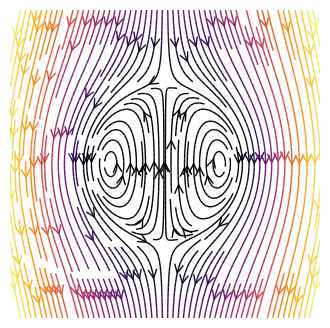
\includegraphics[height=0.3\textwidth]{image/Rising_Stokes.png}
    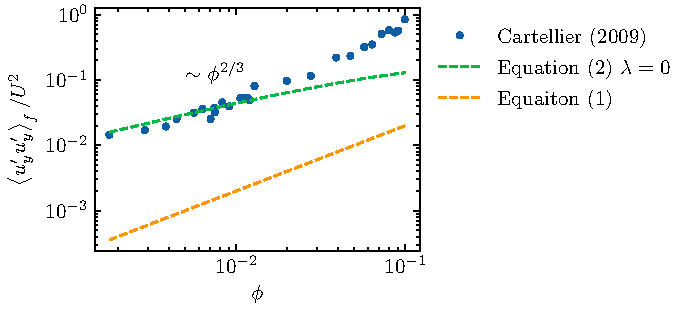
\includegraphics[height=0.3\textwidth]{image/HOMOGENEOUS_NEW/CA/cartellier.pdf}
    \caption{(left) Streamlines of a translating droplet in Stokes flow. 
            (right) Dimensionless Reynolds stress for rising bubbly flows in the direction of gravity. 
            (dots) Experimental results of \cite{cartellier2009induced}. 
            Equation (\ref{eq1}) : Potential flow theory \cite{van1982bubble}. 
            Equation (\ref{eq:results}) Stokes flow theory. 
            }
    \label{fig:wake}
\end{figure}
As can be observed on Figure \ref{fig:wake}, the present theory is in very good agreement with the experimental results of \cite{cartellier2009induced}.  
Direct numerical simulations of rising buoyant emulsions have also been performed (with the code \url{http://basilisk.fr}) for $\lambda = 0.1,1,10$. Good agreement is also obtained. 

In conclusion we provided a \textit{Reynolds stress} closure valid in the dilute Stokes flow regime for arbitrary viscosity ratios. 

\bibliography{Bib/bib_bulles.bib}
\end{document}
